\subsection{Glyph: \glyph{Stimulation}}
\label{sec:stimulation}

A stimulation affects \textbf{positively} the flux of a process represented by the target process.
This stimulation can be, for instance, a catalysis or a positive allosteric regulation. Note that \glyph{catalysis} exists independently in SBGN, see \sect{catalysis}.

\begin{glyphDescription}

\glyphSboTerm
SBO:0000170 ! stimulation

\glyphOrigin
One \glyph{EPN} (\sect{EPNs}) or  \glyph{logical operator} (\sect{logic}).

\glyphTarget
One \glyph{process node} (\sect{PNs}).

\glyphSymbol
The target extremity of a \glyph{stimulation} carries an empty arrowhead, as shown in \fig{stimulation}.

\end{glyphDescription}

\begin{figure}[H]
  \centering
  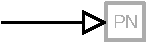
\includegraphics{images/build/stimulation.pdf}
  \caption{The \PD glyph for \glyph{stimulation}.}
  \label{fig:stimulation}
\end{figure}
